\documentclass[aspectratio=169,10pt]{beamer}

\usetheme{Madrid}
\setbeamertemplate{navigation symbols}{}
\setbeamertemplate{footline}[frame number]
\usepackage{hyperref}
\usepackage{amsmath}
\usepackage{amssymb}
\usepackage{array}
\usepackage{booktabs}
\usepackage{graphicx}
\usepackage{tabularx}
\usepackage{tikz}
\usetikzlibrary{arrows.meta,calc,positioning}

\graphicspath{{../../figures_intensity/}}

\definecolor{LectureBlue}{RGB}{13,76,100}
\definecolor{LectureTeal}{RGB}{0,118,122}
\definecolor{LectureGold}{RGB}{194,142,37}
\definecolor{Slate}{RGB}{58,68,84}
\definecolor{SoftGray}{RGB}{245,247,249}

\setbeamercolor{title}{fg=LectureBlue}
\setbeamercolor{subtitle}{fg=Slate}
\setbeamercolor{frametitle}{fg=LectureBlue,bg=LectureBlue!8}
\setbeamercolor{structure}{fg=LectureBlue}
\setbeamercolor{block title}{fg=white,bg=LectureBlue}
\setbeamercolor{block body}{fg=black,bg=SoftGray}
\setbeamercolor{alerted text}{fg=LectureGold}

\renewcommand{\arraystretch}{1.12}

\title{Intensity Transformation and Spatial Filtering}
\subtitle{Spatial \& Frequency Domain Neighborhood Processing and Anti-Aliasing in Deep Learning}
\author{Data Science Lectures}
\date{May 2026}

\begin{document}

% Title Page
\begin{frame}[plain]
\begin{columns}[c,onlytextwidth]
\column{0.58\textwidth}
{\usebeamerfont{title}\color{LectureBlue}\inserttitle\par}
\vspace{0.4em}
{\usebeamerfont{subtitle}\color{Slate}\insertsubtitle\par}
\vspace{1.5em}
{\small \insertauthor \hfill \insertdate}

\column{0.38\textwidth}
\includegraphics[width=\linewidth]{ex_over.png}
\end{columns}
\end{frame}

% Contents Outline
\begin{frame}{Outlines}
\begin{itemize}
\item \textbf{Intensity Transformation (Point Processing)}
  \begin{itemize}
  \item Point transformations: Negative and Piecewise linear functions
  \item Histogram processing: Equalization (HE) and CLAHE
  \end{itemize}
\vspace{0.4em}
\item \textbf{Spatial Domain Filtering}
  \begin{itemize}
  \item Linear spatial filtering (Correlation vs. Convolution)
  \item Smoothing filters (Box, Gaussian, Median, $\alpha$-trimmed mean)
  \item Sharpening filters (discrete Laplacian, Sobel operators)
  \end{itemize}
\vspace{0.4em}
\item \textbf{Frequency Domain Filtering}
  \begin{itemize}
  \item Fourier Series and Fourier Transforms
  \item Discrete Fourier Transform (DFT, 2D FFT) and Aliasing
  \item Frequency Domain Filters (Lowpass, Highpass, Notch) 
  \item Radon Transform
  \end{itemize}
\vspace{0.4em}
\item \textbf{Deep Learning Perspectives}
  \begin{itemize}
  \item Shift-invariance violations and anti-aliasing via BlurPool
  \item Oversmoothing in Vision Transformers and FeatScale analysis
  \end{itemize}
\end{itemize}
\end{frame}

% ==================== SECTION 1 ====================
\section{Intensity Transformation}
\begin{frame}
\centering
\vspace{0.25\textheight}
{\Huge Intensity Transformation (Point Processing)}
\end{frame}

\begin{frame}{Spatial Domain vs. Frequency Domain}
There are two fundamental approaches to perform image processing:
\vspace{0.8em}
\begin{itemize}
\item \textbf{Spatial Domain}: refers to the image plane itself. Processing methods in this category operate directly on the pixels of the image.
\vspace{0.5em}
\item \textbf{Frequency Domain}: refers to transforming an image using a Fourier transform, performing filtering operations in the frequency spectrum, and reconstructing the image back into the spatial domain with an inverse Fourier transform.
\end{itemize}
\vspace{1em}
\begin{block}{Spatial Domain Operations}
All point processing and spatial domain filtering operations are modeled by:
\[
g(x,y) = T[f(x,y)]
\]
where $f(x,y)$ is the input image, $g(x, y)$ is the output image, and $T$ is an operator on $f$ defined over a neighborhood of point $(x,y)$.
\end{block}
\end{frame}

\begin{frame}{Point Transformation}
\begin{columns}[T,onlytextwidth]
\column{0.55\textwidth}
\begin{itemize}
\item The smallest possible neighborhood is of size $1 \times 1$.
\item In this case, $T$ becomes a grey-level mapping function (or look-up table) of a single variable:
\[
s = T(r)
\]
where:
\begin{itemize}
\item $r = f(x,y)$ represents the input pixel value.
\item $s = g(x,y)$ represents the output pixel value.
\end{itemize}
\item Point transformations alter the contrast and brightness of individual pixels, independent of their neighbors.
\end{itemize}

\column{0.40\textwidth}
\centering
\includegraphics[width=0.9\linewidth]{ex_other.png}
\par\vspace{0.5em}{\scriptsize Point Transformation Functions}
\end{columns}
\end{frame}

\begin{frame}{Applications of Point Transformations}
Point transformations are heavily used in medical imaging to enhance visibility:
\vspace{1em}
\begin{columns}[c,onlytextwidth]
\column{0.32\textwidth}
\centering
\includegraphics[height=0.45\textheight]{ex_mam.png}
\par\vspace{0.3em}\tiny{Mammography}

\column{0.32\textwidth}
\centering
\includegraphics[height=0.45\textheight]{ex_spine.png}
\par\vspace{0.3em}\tiny{Spine CT Scan}

\column{0.32\textwidth}
\centering
\includegraphics[height=0.45\textheight]{ex_bean.png}
\par\vspace{0.3em}\tiny{Tissue Contrast Enhancement}
\end{columns}
\end{frame}

\begin{frame}{Negative and Piecewise Linear Transformations}
\begin{columns}[T,onlytextwidth]
\column{0.48\textwidth}
\begin{block}{Negative Transformation}
For an image with intensity levels in the range $[0, L-1]$, the negative transformation is defined as:
\[
s = (L-1) - r
\]
Reversing the intensity values of an image in this way is highly useful for enhancing white/light detail embedded in dark areas (e.g. analysis of calcification in medical mammograms).
\end{block}

\column{0.48\textwidth}
\begin{block}{Piecewise Linear Transformations}
Piecewise linear functions can selectively stretch or compress contrast in specified intensity ranges.
\begin{itemize}
\item \textbf{Contrast Stretching}: maps low-contrast inputs into a wider dynamic range.
\item \textbf{Thresholding}: maps values above a threshold $T$ to white, and values below to black, converting a grayscale image to binary.
\end{itemize}
\end{block}
\end{columns}
\end{frame}

\begin{frame}{Histogram Processing}
\begin{itemize}
\item An image histogram is a graphical representation of the frequency distribution of pixel intensity values.
\item For a digital image with gray levels in the range $[0, L-1]$, the histogram is a discrete function:


\[
h(r_k) = n_k
\]


where $r_k$ is the $k$-th gray level and $n_k$ is the number of pixels in the image having gray level $r_k$.
\item Normalizing the histogram yields the probability of occurrence of gray level $r_k$:


\[
p(r_k) = \frac{n_k}{MN}
\]


where $M \times N$ is the image dimension.
\end{itemize}
\end{frame}

\begin{frame}{Histogram Processing}
\centering
\includegraphics[width=0.95\linewidth]{ex_hist.png}
\par\vspace{0.3em}\tiny{Grayscale Histogram Viz}
\end{frame}



\begin{frame}{Histogram Equalization (HE) - Concept}
\begin{itemize}
\item Histogram Equalization automatically maps intensity levels to achieve a uniform distribution, maximizing global contrast.
\item The transformation function is the Cumulative Distribution Function (CDF):


\[
s_k = T(r_k) = (L-1) \sum_{j=0}^{k} p(r_j) = \frac{L-1}{MN} \sum_{j=0}^{k} n_j
\]


where $\sum p(r_j) = 1$.
\item This mapping is guaranteed to be monotonic, preserving the intensity order.
\end{itemize}
\end{frame}

\begin{frame}{Histogram Equalization (HE) - Visualization}
\centering
\includegraphics[width=0.9\linewidth]{hist_eq.png}
\par\vspace{0.3em}\tiny{Global Histogram Equalization Transfer}
\end{frame}

\begin{frame}{Comparison: Global HE vs. CLAHE}
\small
\begin{tabularx}{\linewidth}{>{\bfseries}p{0.22\linewidth} X}
\toprule
Method & Description \\
\midrule
Global HE & Computes the cumulative distribution function (CDF) across the entire image. Improves overall contrast but can over-amplify noise and wash out details in uneven lighting. \\
\midrule
CLAHE & Divides the image into small local tiles (e.g. $8 \times 8$). Limits contrast amplification to avoid noise, interpolating tile boundaries. \\
\bottomrule
\end{tabularx}

\vspace{1em}
\small
\textbf{CLAHE Explanation:} Contrast Limited Adaptive Histogram Equalization enhances local contrast by working on small regions instead of the whole image. By limiting the amplification of contrast, it reduces noise and preserves fine details, making it especially useful for medical and low-light images.
\end{frame}



\begin{frame}{Comparison: Global HE vs. CLAHE}
\centering
\includegraphics[width=1\linewidth]{ex_hist_eq.png}
\par\vspace{0.3em}\tiny{Comparison of HE and CLAHE}
\end{frame}



% ==================== SECTION 2 ====================
\section{Spatial Filtering}
\begin{frame}
\centering
\vspace{0.25\textheight}
{\Huge Spatial Domain Filtering (Neighborhood Processing)}
\end{frame}

\begin{frame}{Linear Spatial Filtering}
\begin{columns}[T,onlytextwidth]
\column{0.55\textwidth}
\begin{itemize}
\item Spatial filtering replaces the value of each pixel by a function of the pixel value and its neighbors.
\item A linear spatial filter performs a sum-of-products operation between an image $f$ and a filter \textbf{kernel} (or mask, window, impulse response) $h$.
\item The kernel coefficients determine the filter behavior (e.g., smoothing or sharpening).
\end{itemize}

\column{0.40\textwidth}
\centering
\includegraphics[width=\linewidth]{convolve.png}
\par\vspace{0.3em}\tiny{Kernel Sweeping Across Image Grid}
\end{columns}
\end{frame}

\begin{frame}{Cross-Correlation vs. Convolution}
\begin{columns}[T,onlytextwidth]
\column{0.48\textwidth}
\begin{block}{Cross-Correlation}
Slides the kernel directly over the image:
\[
g(i, j) = \sum_{m=-a}^a \sum_{n=-b}^b f(i+m, j+n) h(m, n)
\]
\[
g = f \otimes h
\]
where $h$ is a kernel of size $(2a+1) \times (2b+1)$.
\end{block}
\vspace{0.3em}
\begin{alertblock}{Deep Learning Note}
In deep learning frameworks, standard "convolutional" layers are actually implemented as cross-correlation. Flipping the kernel is not needed because the weights are learned.
\end{alertblock}

\column{0.48\textwidth}
\begin{block}{Convolution}
Flips the kernel both horizontally and vertically before sliding:
\[
g(i, j) = \sum_{m=-a}^a \sum_{n=-b}^b f(i-m, j-n) h(m, n)
\]
\[
g = f * h
\]
Convolution is mathematically associative and commutative, whereas cross-correlation is not.
\end{block}
\end{columns}
\end{frame}
\begin{frame}{Linear Lowpass Filtering (Smoothing)}
Smoothing filters attenuate high-frequency transitions (noise, sharp edges) to blur details.
\vspace{0.8em}
\begin{columns}[T,onlytextwidth]
\column{0.48\textwidth}
\begin{block}{Moving Average (Box) Filter}
Replaces each pixel with the average of its neighbors in a window. A $3 \times 3$ box filter is:


\[
K_{box} = \frac{1}{9} \begin{bmatrix} 1 & 1 & 1 \\ 1 & 1 & 1 \\ 1 & 1 & 1 \end{bmatrix}
\]


\end{block}

\column{0.48\textwidth}
\begin{block}{Gaussian Filter}
Uses weights that decrease exponentially with distance from the center, preserving edges better:


\[
K_{gauss} = \frac{1}{16} \begin{bmatrix} 1 & 2 & 1 \\ 2 & 4 & 2 \\ 1 & 2 & 1 \end{bmatrix}
\]


\end{block}
\end{columns}
\end{frame}

\begin{frame}{Linear Lowpass Filtering (Examples)}
\centering
\includegraphics[width=0.9\linewidth]{filter_mv.png}
\vspace{1em}
\includegraphics[width=0.9\linewidth]{filter_gaussian.png}
\end{frame}

\begin{frame}{Non-linear Lowpass Filtering (Smoothing)}
Non-linear filters use neighborhood ordering instead of weighted sums to reduce noise.
\vspace{0.8em}
\begin{columns}[T,onlytextwidth]
\column{0.48\textwidth}
\begin{block}{Median Filter}
Replaces each pixel with the median value of pixels in the neighborhood.
\begin{itemize}
\item Highly effective at removing \textbf{salt-and-pepper noise} (impulsive spikes).
\item Minimizes blurring of sharp boundaries compared to linear lowpass filters.
\end{itemize}
\end{block}

\column{0.48\textwidth}
\begin{block}{$\alpha$-Trimmed Mean Filter}
A hybrid between mean and median filters:
\begin{enumerate}
\item Sorts pixel values in the neighborhood.
\item Discards $\alpha\%$ of the smallest and largest values.
\item Computes the mean of the remaining pixels.
\end{enumerate}
Excellent for noise models containing both Gaussian and impulse noise.
\end{block}
\end{columns}
\end{frame}

\begin{frame}{Non-linear Lowpass Filtering (Smoothing)}
\centering
\includegraphics[width=1\linewidth]{filter_nonlinear.png}
\end{frame}



\begin{frame}{Linear Highpass Filtering: The Laplacian Operator}
Highpass filters amplify high-frequency changes, useful for edge detection and sharpening.
\vspace{0.8em}

\begin{itemize}
\item The \textbf{Laplacian} ($\nabla^2$) is a second-order derivative operator:


\[
\nabla^2 f = \frac{\partial^2 f}{\partial x^2} + \frac{\partial^2 f}{\partial y^2}
\]


\item Discrete finite-difference approximation:
\begin{align*}
\nabla^2 f(x, y) \approx & f(x+1, y) + f(x-1, y) \\
& + f(x, y+1) + f(x, y-1) - 4f(x, y)
\end{align*}
\item This corresponds to the convolution kernel:


\[
K_{\nabla^2} = \begin{bmatrix} 0 & 1 & 0 \\ 1 & -4 & 1 \\ 0 & 1 & 0 \end{bmatrix} 
\quad \text{or} \quad
\begin{bmatrix} 1 & 1 & 1 \\ 1 & -8 & 1 \\ 1 & 1 & 1 \end{bmatrix}
\]


\end{itemize}
\end{frame}

\begin{frame}{The Laplacian Operator: Visuals}
\centering
\includegraphics[width=0.55\linewidth]{highpass.png}
\end{frame}

\begin{frame}{The Laplacian Operator: Visuals}
\centering
\includegraphics[width=1\linewidth]{laplacian.png}
\end{frame}



\begin{frame}{Laplacian Applications in Signal Processing}
\begin{columns}[c,onlytextwidth]
\column{0.58\textwidth}
\begin{itemize}
\item The Laplacian is sensitive to fine detail and noise, making it ideal for edge enhancement.
\item \textbf{Image Sharpening}: subtract the Laplacian from the original image to restore blurry details:
\[
g(x,y) = f(x,y) - \nabla^2 f(x,y)
\]
\item \textbf{EEG Reference Preprocessing}: used to spatial-filter multi-channel EEG signals to localize source activity.
\end{itemize}

\column{0.38\textwidth}
\centering
\includegraphics[width=\linewidth]{ex_laplacian_eeg.png}
\par\vspace{0.3em}\tiny{EEG Channel Laplacian Preprocessing}
\end{columns}
\end{frame}

\begin{frame}{Linear Highpass Filtering: The Sobel Operator}
\begin{columns}[T,onlytextwidth]
\column{0.55\textwidth}
\begin{itemize}
\item The first derivative of a 2D image is represented by the gradient vector:
\[
\nabla f = \left[ \frac{\partial f}{\partial x}, \frac{\partial f}{\partial y} \right]^T
\]
\item The gradient magnitude indicates edge strength:
\[
|\nabla f| = \sqrt{\left(\frac{\partial f}{\partial x}\right)^2 + \left(\frac{\partial f}{\partial y}\right)^2}
\]
\item The \textbf{Sobel filter} approximates these derivatives using two convolution kernels:
\[
K_x = \begin{bmatrix} -1 & 0 & 1 \\ -2 & 0 & 2 \\ -1 & 0 & 1 \end{bmatrix}, \quad K_y = \begin{bmatrix} -1 & -2 & -1 \\ 0 & 0 & 0 \\ 1 & 2 & 1 \end{bmatrix}
\]
\end{itemize}

\column{0.40\textwidth}
\centering
\includegraphics[width=0.8\linewidth]{sobel.png}

\end{columns}
\end{frame}

\begin{frame}{The Sobel Operator: Visuals}
\centering
\includegraphics[width=1\linewidth]{ex_sobel2.png}
\end{frame}

% ==================== SECTION 3 ====================
\section{Frequency Domain Filtering}
\begin{frame}
\centering
\vspace{0.25\textheight}
{\Huge Frequency Domain Filtering (Fourier Transforms)}
\end{frame}

\begin{frame}{Why Use the Frequency Domain?}
\begin{itemize}
\item \textbf{Intuitive Interpretation}: Provides a clear understanding of what "smoothing" (lowpass filtering) and "edge sharpening" (highpass filtering) mean in terms of frequency components.
\vspace{0.4em}
\item \textbf{Computational Efficiency}: Direct spatial convolution with a large kernel of size $W \times W$ requires $O(W^2)$ multiplications per pixel.
\vspace{0.4em}
\item \textbf{Convolution Theorem}: Spatial convolution is equivalent to element-wise multiplication in the frequency domain:
\[
f(x,y) * h(x,y) \iff F(u,v) \cdot H(u,v)
\]
Using the Fast Fourier Transform (FFT), this reduces computation to $O(N^2 \log N)$ operations for an $N \times N$ image, regardless of kernel size.
\end{itemize}
\end{frame}

\begin{frame}{Fourier Series and the Continuous Fourier Transform}
\begin{columns}[T,onlytextwidth]
\column{0.48\textwidth}
\begin{block}{Fourier Series}
Any periodic function $f(t)$ with period $T$ can be decomposed into an infinite sum of sines and cosines (or complex exponentials):
\[
f(t) = \sum_{n=-\infty}^{\infty} c_n e^{i \frac{2\pi n}{T} t}
\]
where the coefficients $c_n$ are given by:
\[
c_n = \frac{1}{T} \int_{-T/2}^{T/2} f(t) e^{-i \frac{2\pi n}{T} t} dt
\]
\end{block}

\column{0.48\textwidth}
\begin{block}{Continuous Fourier Transform}
For non-periodic functions, letting $T \to \infty$ yields the continuous Fourier transform:
\[
F(\mu) = \int_{-\infty}^{\infty} f(t) e^{-i 2\pi\mu t} dt
\]
Reconstruction (Inverse Transform):
\[
f(t) = \int_{-\infty}^{\infty} F(\mu) e^{i 2\pi\mu t} d\mu
\]
where $t$ represents time (or space) and $\mu$ represents frequency.
\end{block}
\end{columns}
\end{frame}

\begin{frame}{Discrete Fourier Transform (DFT)}
Images are discrete arrays. To process them, we sample the continuous Fourier transform.
\vspace{0.8em}
\begin{columns}[T,onlytextwidth]
\column{0.55\textwidth}
\begin{itemize}
\item \textbf{Nyquist-Shannon Sampling Theorem}: To prevent aliasing, the sampling rate $f_s$ must exceed twice the maximum frequency present in the continuous signal:
\[
f_s > 2 f_{max}
\]
\item \textbf{1D and 2D Discrete Fourier Transform}:
\[
F_m = \sum_{n=0}^{M-1} f[n] e^{-i \frac{2\pi n m}{M}}
\]
\[
F[u,v] = \sum_{x=0}^{N-1} \sum_{y=0}^{M-1} f[x, y] e^{-j 2\pi \left(\frac{ux}{N} + \frac{vy}{M}\right)}
\]
\end{itemize}

\column{0.40\textwidth}
\begin{block}{Aliasing}
Undersampling causes replicas of the spectrum to overlap in the frequency domain, distorting high-frequency patterns (e.g. Moir\'e patterns).
\end{block}
\end{columns}
\end{frame}

\begin{frame}{Amplitude vs. Phase in Image Spectrum}
The Fourier transform result $F(u,v)$ is complex-valued: $F(u,v) = |F(u,v)|e^{j\phi(u,v)}$.

Animation: \href{https://www.youtube.com/watch?v=MA2y_2YySq0}{\textcolor{red}{Animation click here}}
\vspace{0.8em}
\begin{columns}[T,onlytextwidth]
\column{0.48\textwidth}
\begin{block}{Amplitude (Magnitude) Spectrum}
\[
|F(u,v)| = \sqrt{\text{Re}(F)^2 + \text{Im}(F)^2}
\]
\begin{itemize}
\item Represents the relative prominence of the different frequencies.
\item Stores information about the overall textures, brightness, and noise.
\end{itemize}
\end{block}

\column{0.48\textwidth}
\begin{block}{Phase Spectrum}
\[
\phi(u,v) = \arctan\left( \frac{\text{Im}(F)}{\text{Re}(F)} \right)
\]
\begin{itemize}
\item Represents the alignment and relative displacement of the sinusoidal waves.
\item Carries essential geometric information (where edges, shapes, and structural layout reside).
\end{itemize}
\end{block}
\end{columns}
\end{frame}

\begin{frame}{Filtering in the Frequency Domain}
Frequency domain filtering modifies image frequencies by multiplying the image spectrum:
\[
f'(x,y) = \text{Real}\left[ \mathcal{F}^{-1}\Big(F(u,v) \cdot H(u,v)\Big) \right]
\]
where $F(u,v)$ is the image spectrum, $H(u,v)$ is the filter transfer function, and $f'(x,y)$ is the filtered image.
\vspace{0.8em}
\begin{columns}[T,onlytextwidth]
\column{0.32\textwidth}
\begin{block}{Lowpass Filter}
Attenuates high frequencies, preserving low frequencies. Removes noise but blurs edges.
\end{block}

\column{0.32\textwidth}
\begin{block}{Highpass Filter}
Attenuates low frequencies, preserving high frequencies. Sharpens edges and discards uniform lighting.
\end{block}

\column{0.32\textwidth}
\begin{block}{Notch Filter}
Attenuates specific frequency spikes. Highly effective at removing periodic stripes or noise.
\end{block}
\end{columns}
\end{frame}


\begin{frame}{Lowpass Filtering: Visuals}
\centering
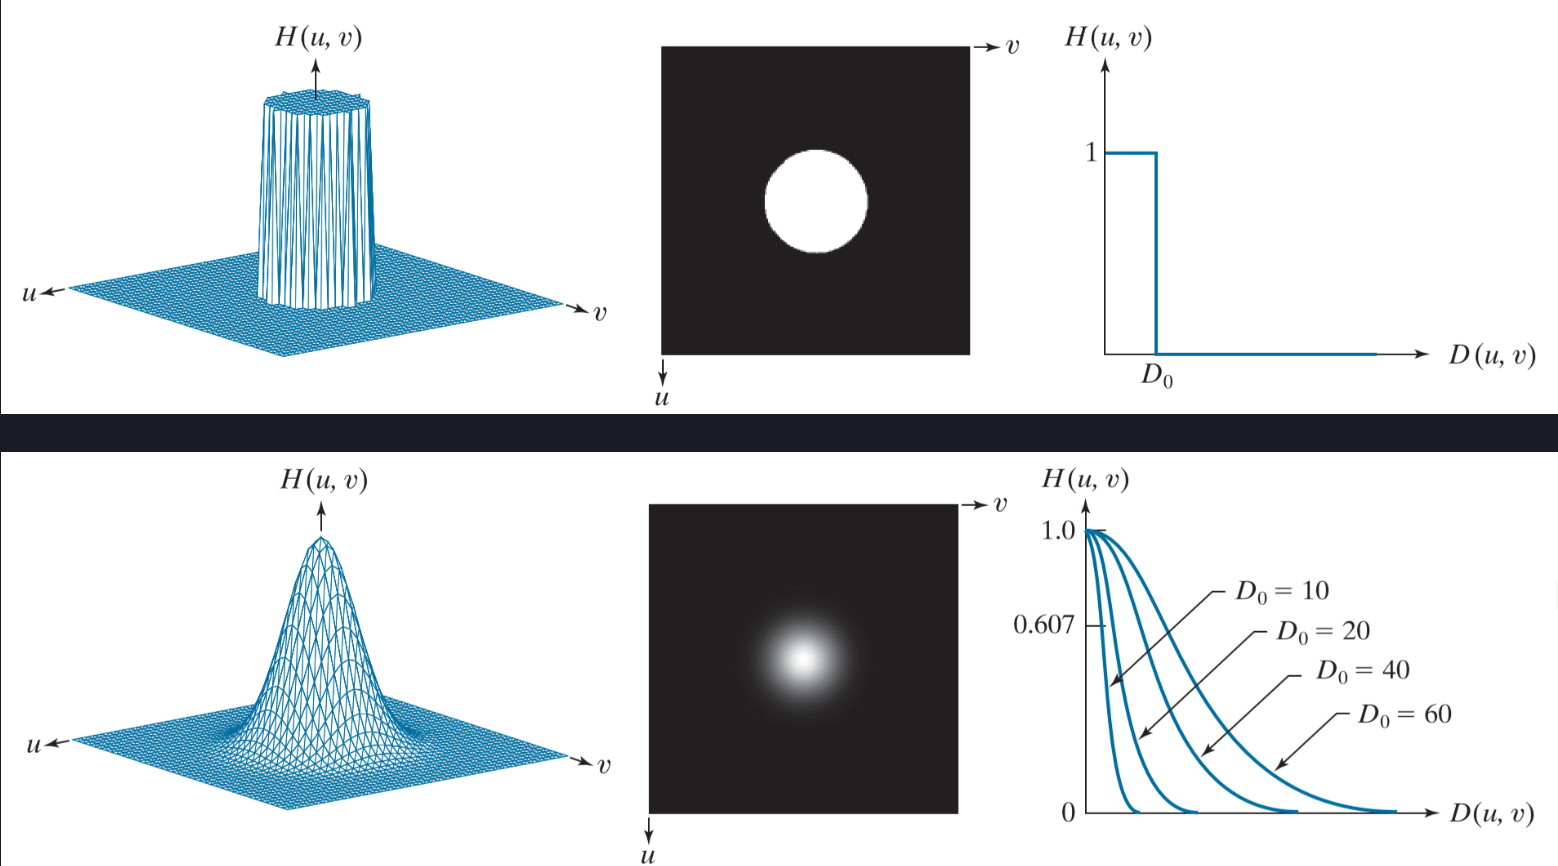
\includegraphics[width=0.9\linewidth]{freq_lowpass.png}
\end{frame}

\begin{frame}{Highpass Filtering: Visuals}
\centering
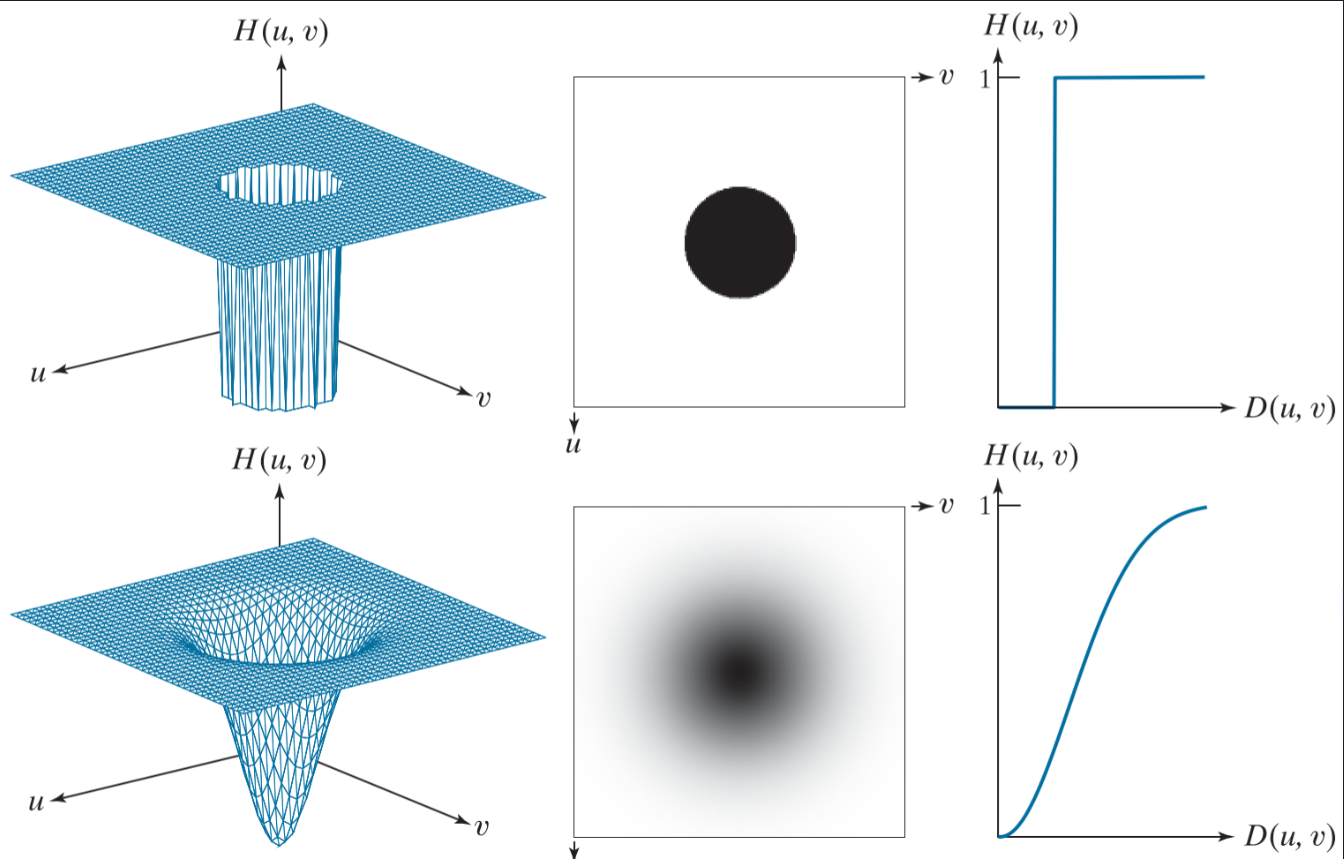
\includegraphics[width=0.8\linewidth]{freq_highpass.png}
\end{frame}

\begin{frame}{Notch Filtering: Visuals}
\centering
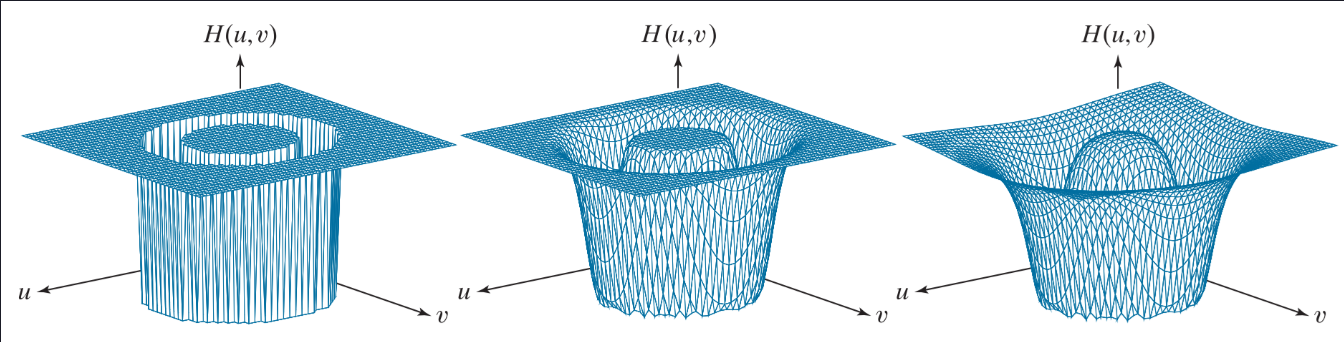
\includegraphics[width=1\linewidth]{freq_notch.png}
\end{frame}

\begin{frame}{Computed Tomography (CT) and the Radon Transform}
\begin{columns}[T,onlytextwidth]
\column{0.55\textwidth}
\begin{itemize}
\item CT scanners acquire 1D projections at various angles $\theta$.
\item \textbf{Radon Transform}: computes line integrals of $f(x,y)$ along lines $x' = x\sin\theta - y\cos\theta$:
\[
R(x', \theta) = \iint f(x,y) \delta\Big[x'-(x\sin\theta - y\cos\theta)\Big] dxdy
\]
\item \textbf{Fourier Slice Theorem}: The 1D Fourier transform of a projection at angle $\theta$ is equal to a 2D radial slice of the 2D Fourier transform of the object $f(x,y)$ at the same angle.
\item Used in Filtered Backprojection (FBP) for CT image reconstruction.
\end{itemize}
Animation: \href{https://www.youtube.com/watch?v=MA2y_2YySq0&t=8s}{\textcolor{red}{Radon transform animation click here}}
\column{0.40\textwidth}
\centering
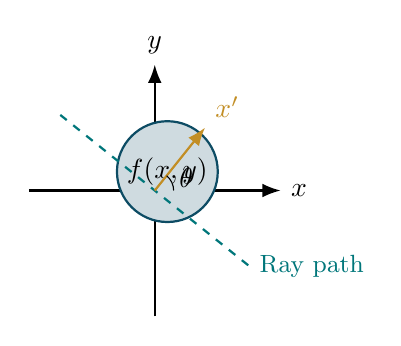
\begin{tikzpicture}[scale=0.8,>=Latex]
\draw[->,thick] (-2,0) -- (2,0) node[right] {$x$};
\draw[->,thick] (0,-2) -- (0,2) node[above] {$y$};
\draw[fill=LectureBlue!20,draw=LectureBlue,thick] (0.2,0.3) circle (0.8);
\node at (0.2,0.3) {$f(x,y)$};
\draw[dashed,LectureTeal,thick] (-1.5,1.2) -- (1.5,-1.2) node[right,font=\small] {Ray path};
\draw[->,thick,LectureGold] (0,0) -- (0.8,1.0) node[above right] {$x'$};
\draw (0.3,0) arc (0:51:0.3);
\node at (0.5,0.2) {$\theta$};
\end{tikzpicture}

\end{columns}


\end{frame}

\begin{frame}{Radon Transform: Visuals}
\centering
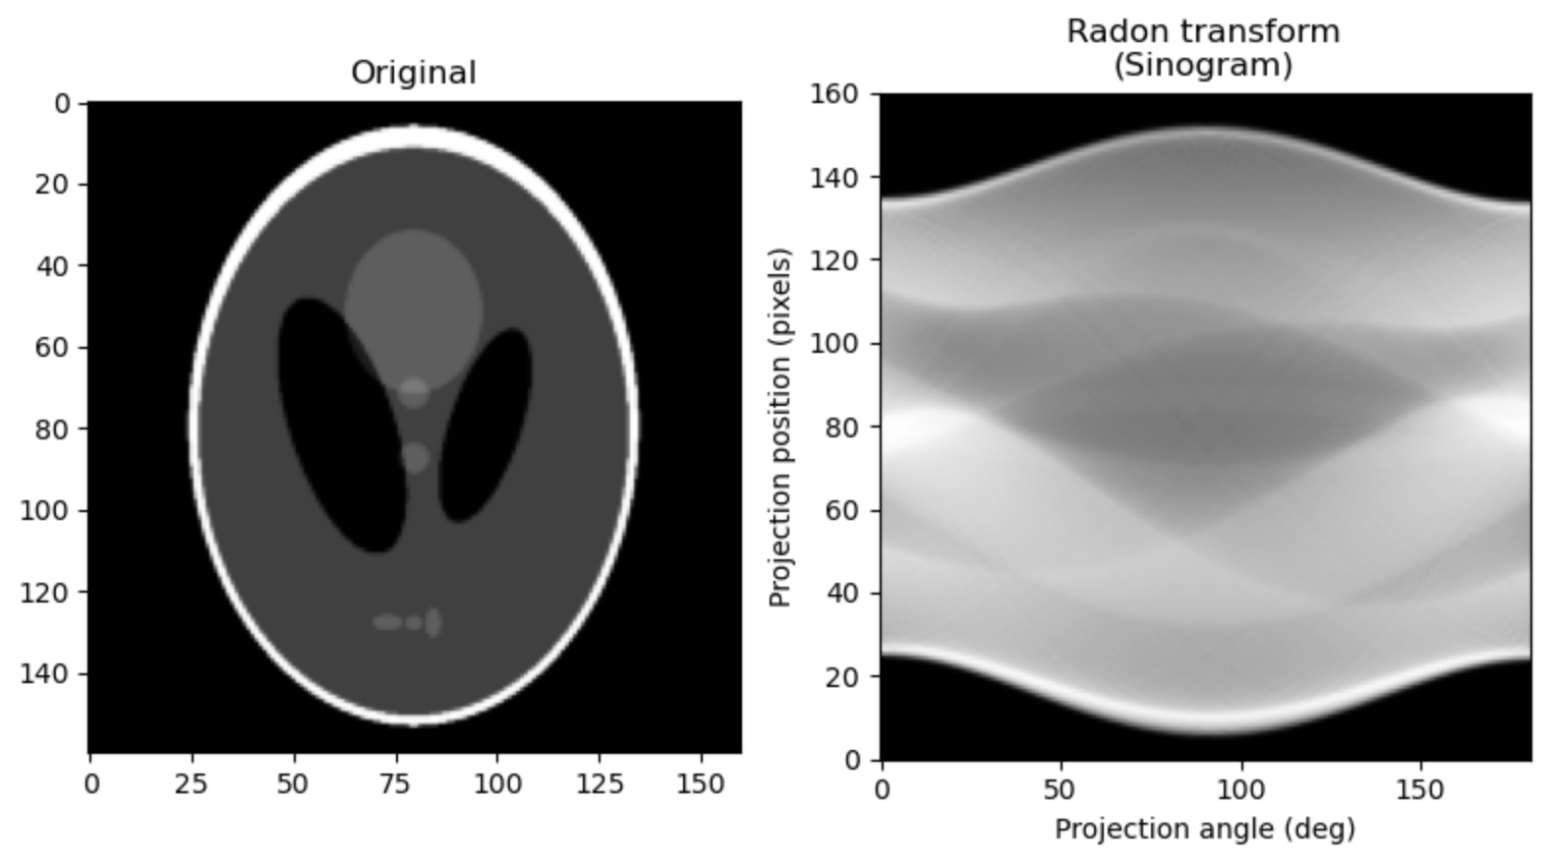
\includegraphics[width=1\linewidth]{freq_radon.png}
\end{frame}

\begin{frame}{Radon Transform: Visuals}
\centering
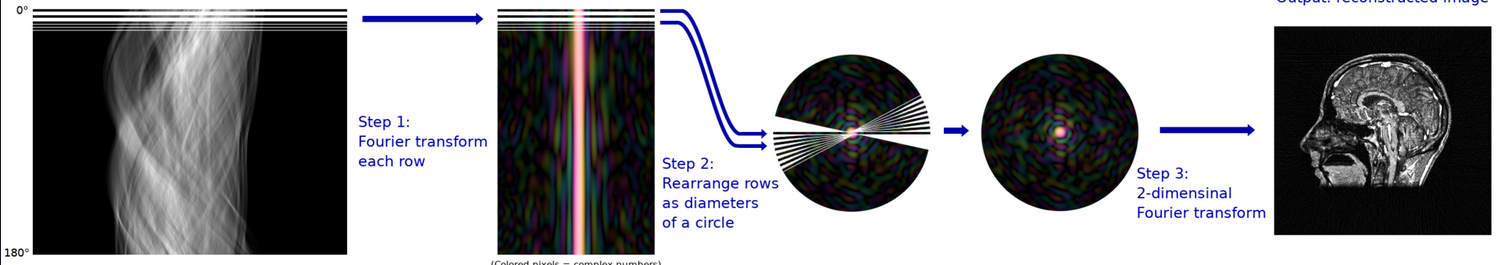
\includegraphics[width=1\linewidth]{freq_radon_flow.png}
\end{frame}

% ==================== SECTION 4 ====================
\section{Deep Learning Perspectives}
\begin{frame}
\centering
\vspace{0.25\textheight}
{\Huge Deep Learning Perspectives (Aliasing \& Frequency Analysis)}
\end{frame}

\begin{frame}{CNNs are NOT Shift-Invariant}

\begin{itemize}
    \item Shifting an image by just one pixel can drastically change classification outputs.
    \item Downsampling layers (Max-Pooling, Average Pooling, Strided Convolutions) violate the Nyquist sampling rate.
    \item Downsampling without proper prefiltering introduces \textbf{aliasing} in internal feature maps.
\end{itemize}

\vfill
\begin{center}
    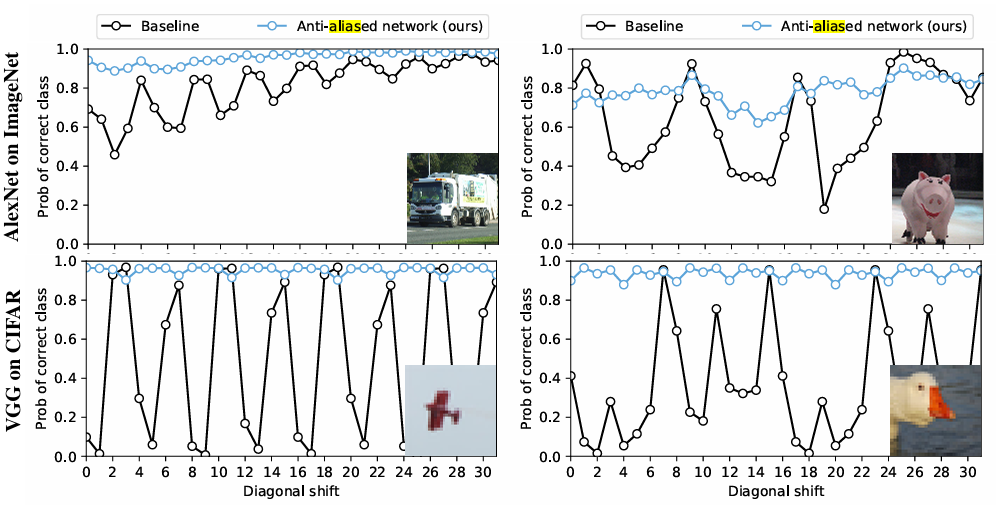
\includegraphics[width=0.7\linewidth]{dl_shift.png} \\
    \vspace{0.3em}
    \tiny{Shift Instability in Standard CNNs}
\end{center}

\end{frame}

\begin{frame}{Anti-Aliasing in Deep Learning: BlurPool}
To restore shift-invariance, CNN downsampling layers must incorporate anti-aliasing.
\vspace{0.8em}

\begin{block}{The BlurPool Strategy}
Instead of combining max-filtering and downsampling in one strided step, the operation is split:
\begin{enumerate}
\item Apply Max-filtering with stride = 1 (preserves spatial resolution).
\item Apply a low-pass filter (e.g. $3 \times 3$ binomial blur kernel).
\item Subsample (stride = 2).
\end{enumerate}
This satisfies Nyquist and restores shift-equivariance in hidden representations.
\end{block}
\end{frame}

\begin{frame}{Anti-Aliasing in Deep Learning: BlurPool}
\begin{figure}[H]
\centering
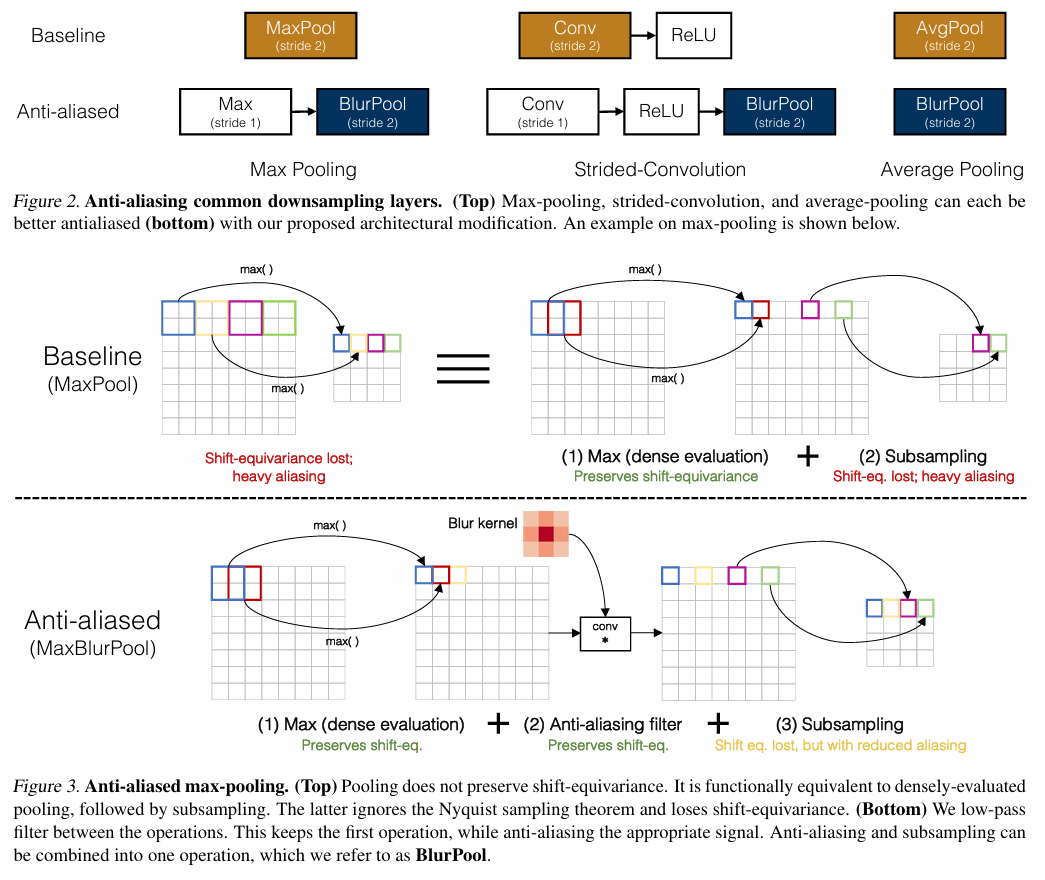
\includegraphics[width=0.6\linewidth]{dl_blurpool.png}

\end{figure}
\end{frame}

\begin{frame}{Anti-Aliasing in Deep Learning: BlurPool}
\begin{figure}[H]
\centering
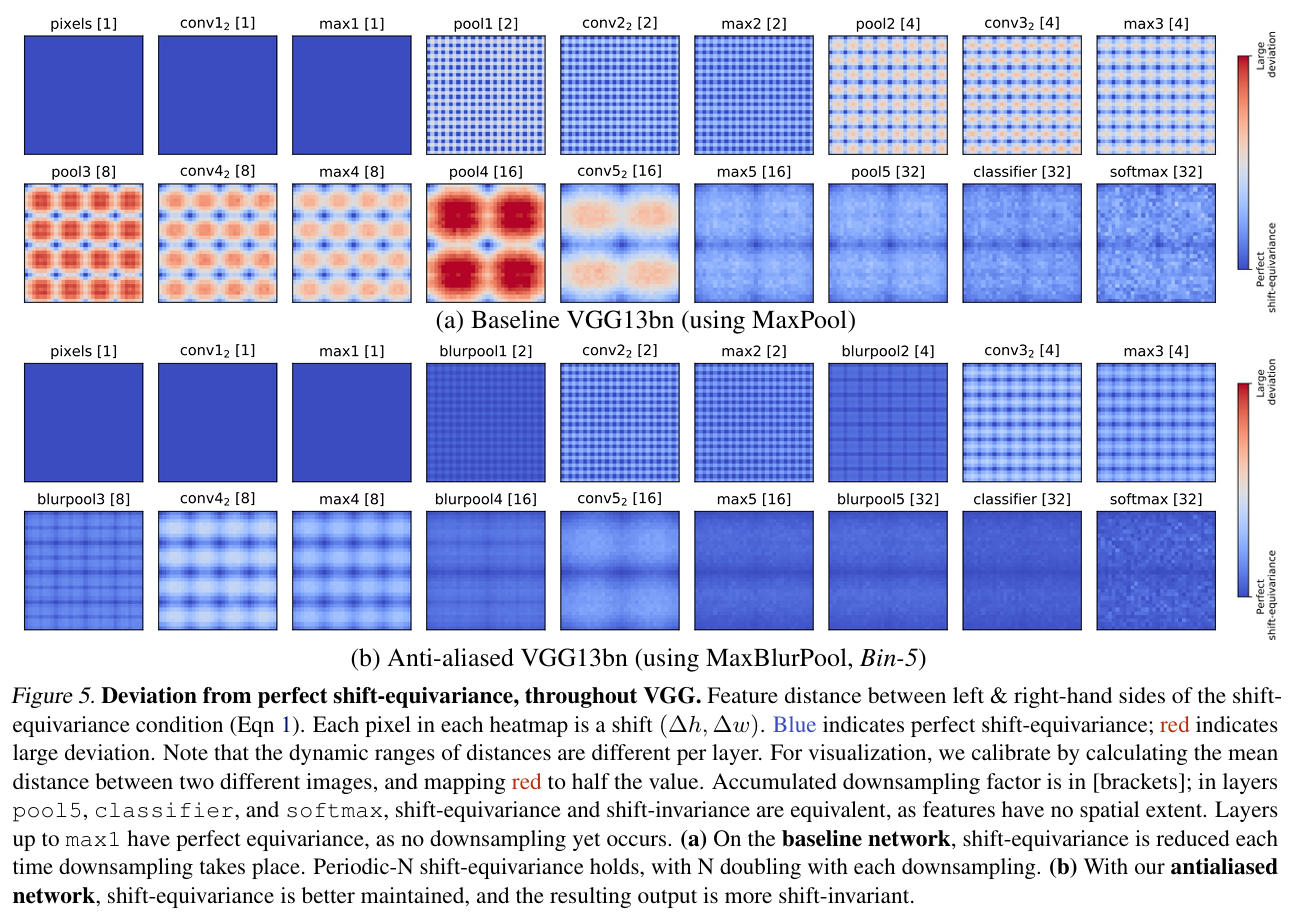
\includegraphics[width=0.7\linewidth]{dl_blurresults.png}

\end{figure}
\end{frame}

\begin{frame}{Oversmoothing in Vision Transformers (ViTs)}
Vision Transformers analyze images using Self-Attention and Multi-Layer Perceptrons.
\vspace{0.8em}

\begin{itemize}
\item Self-Attention layers act as \textbf{lowpass filters}, smoothing the features of image patches.
\vspace{0.5em}
\item In deep ViTs, the repeated cascading of self-attention leads to \textbf{oversmoothing}—patch features collapse and become nearly identical, degrading representation capacity.
\end{itemize}
\end{frame}

\begin{frame}{Oversmoothing in Vision Transformers (ViTs)}
\begin{figure}[H]
\centering
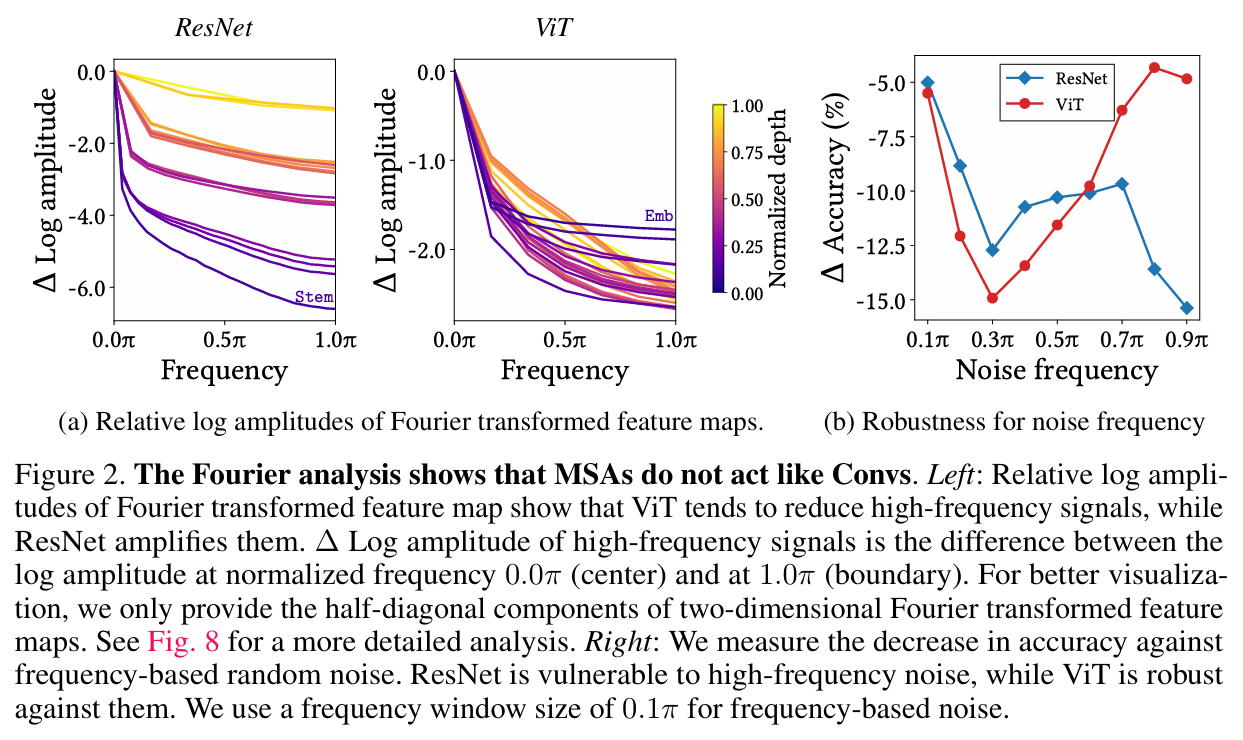
\includegraphics[width=0.8\linewidth]{dl_vit_lowpass.png}
\end{figure}
\end{frame}

\begin{frame}{Preventing Oversmoothing: FeatScale}
To combat representation collapse, Fourier domain analysis is applied directly to token features.


\begin{block}{The FeatScale Method}
\begin{itemize}
\item FeatScale regulates the frequency spectrum of token representations inside deep transformer blocks.
\item By analyzing features in the frequency domain, it dynamically rescales spatial frequencies to amplify high-frequency components.
\item This prevents oversmoothing and preserves patch diversity, leading to improved accuracy.
\end{itemize}
\end{block}
\begin{center}
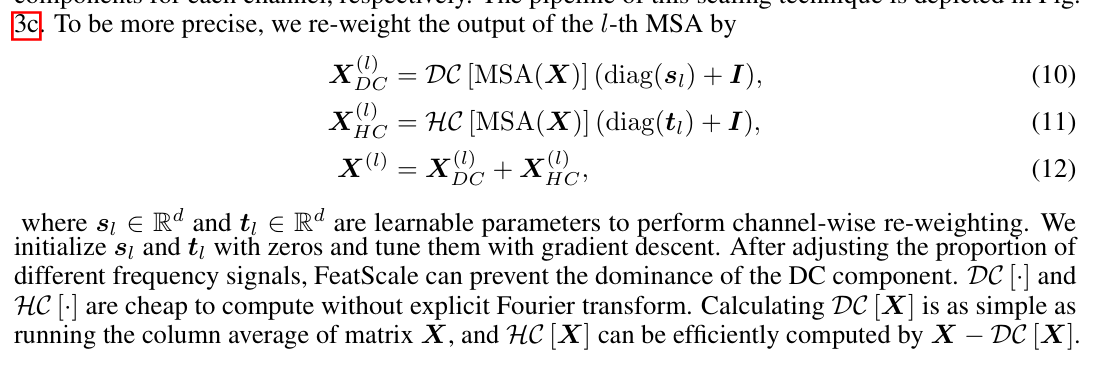
\includegraphics[width=0.85\linewidth]{dl_featscale.png}
\end{center}
\end{frame}

\begin{frame}{Preventing Oversmoothing: FeatScale}

\begin{center}

    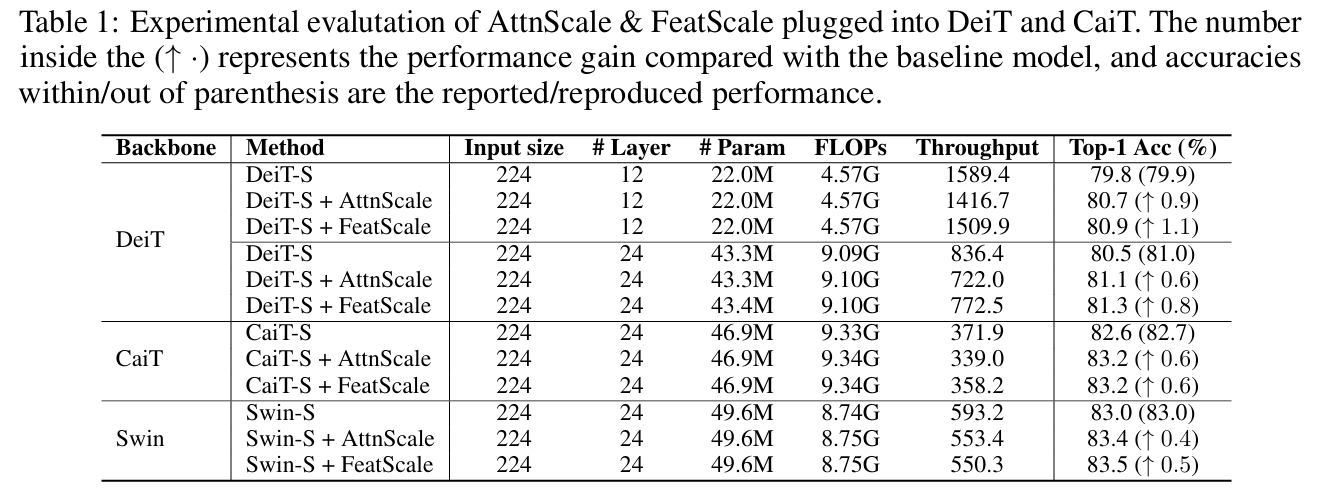
\includegraphics[width=1\linewidth]{dl_featscale_results.png}
    
    \
\end{center}

\end{frame}


% ==================== SECTION 5 ====================
\section{Other Applications}
\begin{frame}
\centering
\vspace{0.25\textheight}
{\Huge Other Applications}
\end{frame}

\begin{frame}{Neuroscience and Astronomy}
\begin{columns}[T,onlytextwidth]
\column{0.48\textwidth}
\begin{block}{EEG Signal Analysis}
\begin{itemize}
\item In neuroscience, multi-channel EEG electrodes measure brain electrical activity.
\item Fast Fourier Transform (FFT) is applied to decompose continuous brain waves into distinct frequency bands:
  \begin{itemize}
  \item \textbf{Delta ($\delta$)}: $< 4$ Hz (Deep sleep)
  \item \textbf{Theta ($\theta$)}: $4 - 8$ Hz (Drowsiness)
  \item \textbf{Alpha ($\alpha$)}: $8 - 12$ Hz (Relaxed alert)
  \item \textbf{Beta ($\beta$)}: $12 - 30$ Hz (Active thinking)
  \end{itemize}
\item Used to identify sleep cycles and cognitive states.
\end{itemize}
\end{block}

\column{0.48\textwidth}
\begin{block}{Radio Astronomy Interferometry}
\begin{itemize}
\item Radio telescopes observe celestial objects using arrays of dishes spread across continents (interferometry).
\item Due to sparse spatial sampling, the raw data is incomplete.
\item Fourier synthesis is used to reconstruct images (e.g. Event Horizon Telescope black hole imaging) by solving phase retrieval and sparse inverse Fourier problems.
\end{itemize}
\end{block}
\end{columns}
\end{frame}

\begin{frame}{Summary}
\begin{itemize}
\item \textbf{Intensity Transformations} (Negative, Piecewise linear, Histogram processing) manipulate contrast and gray levels directly at the pixel level.
\vspace{0.5em}
\item \textbf{Spatial Domain Filtering} uses convolution/correlation kernels to perform local neighborhood operations (smoothing, Laplacian/Sobel edge detection).
\vspace{0.5em}
\item \textbf{Frequency Domain Filtering} transforms spatial images into sinusoidal components, enabling efficient filtering (Lowpass, Highpass, Notch) and CT reconstruction (Radon/Fourier Slice Theorem).
\vspace{0.5em}
\item \textbf{Classical Image Processing in Deep Learning}: Aliasing and frequency oversmoothing continue to be critical challenges, addressed by architectural components like BlurPool and FeatScale.
\end{itemize}
\end{frame}

\end{document}
